\documentclass[12pt,a4paper]{article}

% ─── Page Layout ───────────────────────────────────────────────────────────────
\usepackage[a4paper, margin=0.8in, headheight=14pt]{geometry}

% ─── Fonts (XeLaTeX) ───────────────────────────────────────────────────────────
\usepackage{fontspec}
\usepackage{unicode-math}
\setmainfont{TeX Gyre Pagella}
\setmonofont[Scale=0.88]{TeX Gyre Cursor}
\setmathfont{Latin Modern Math}

% ─── Packages ──────────────────────────────────────────────────────────────────
\usepackage{xcolor}
\usepackage{colortbl}
\usepackage{titlesec}
\usepackage{enumitem}
\usepackage{tabularx}
\usepackage{booktabs}
\usepackage{array}
\usepackage{amsmath}
\usepackage{tikz}
\usetikzlibrary{shapes.geometric, arrows.meta, positioning, calc, fit, decorations.pathreplacing}
\usepackage{tcolorbox}
\tcbuselibrary{skins, breakable}
\usepackage{hyperref}
\usepackage{fancyhdr}
\usepackage{graphicx}
\usepackage{microtype}
\hyphenpenalty=10000
\exhyphenpenalty=10000
\sloppy
\usepackage{caption}
\usepackage{setspace}
\usepackage{multirow}
\usepackage{tocloft}

% ─── Q&A helper ────────────────────────────────────────────────────────────────
\newcommand{\Q}[1]{\textbf{#1}\par\noindent\ignorespaces}

% ─── Colour Palette ────────────────────────────────────────────────────────────
\definecolor{myred}{RGB}{196,30,58}
\definecolor{mydark}{RGB}{30,30,50}
\definecolor{mygreen}{RGB}{14,120,80}
\definecolor{myteal}{RGB}{0,130,140}
\definecolor{myamber}{RGB}{180,100,0}
\definecolor{mypurple}{RGB}{100,30,160}
\definecolor{mygray}{RGB}{246,247,249}
\definecolor{mgframe}{RGB}{180,185,200}
\definecolor{watermark}{RGB}{145,150,170}
\definecolor{hdrred}{RGB}{250,232,235}
\definecolor{hdrgreen}{RGB}{220,244,233}
\definecolor{hdrteal}{RGB}{220,242,244}
\definecolor{hdramber}{RGB}{253,242,215}
\definecolor{hdrpurple}{RGB}{238,228,255}
\definecolor{hdrgray}{RGB}{238,240,245}
\definecolor{rowalt}{RGB}{250,251,253}

% ─── Section Formatting ────────────────────────────────────────────────────────
\titleformat{\section}
  {\large\bfseries\color{myred}}{\thesection.}{0.5em}{}
  [\vspace{1pt}{\color{myred}\rule{\linewidth}{0.8pt}}]
\titleformat{\subsection}
  {\normalsize\bfseries\color{myteal}}{\thesubsection}{0.5em}{}
\titlespacing*{\section}{0pt}{18pt}{7pt}
\titlespacing*{\subsection}{0pt}{11pt}{4pt}

% ─── Paragraph ─────────────────────────────────────────────────────────────────
\setlength{\parindent}{0pt}
\setlength{\parskip}{4pt}

% ─── TOC Styling ───────────────────────────────────────────────────────────────
\renewcommand{\cfttoctitlefont}{\large\bfseries\color{myred}}
\renewcommand{\cftaftertoctitle}{\par\noindent{\color{myred}\rule{\linewidth}{0.8pt}}}
\setlength{\cftbeforetoctitleskip}{0pt}
\setlength{\cftaftertoctitleskip}{6pt}
\renewcommand{\cftsecfont}{\normalsize\bfseries\color{mydark}}
\renewcommand{\cftsecpagefont}{\normalsize\bfseries\color{mydark}}
\renewcommand{\cftsecleader}{\cftdotfill{\cftdotsep}}
\setlength{\cftbeforesecskip}{7pt}
\renewcommand{\cftsubsecfont}{\small\color{mydark}}
\renewcommand{\cftsubsecpagefont}{\small\color{mydark}}
\setlength{\cftbeforesubsecskip}{3pt}
\setlength{\cftsubsecindent}{1.4em}

% ─── Table helpers ─────────────────────────────────────────────────────────────
\renewcommand{\arraystretch}{1.45}
\setlength{\tabcolsep}{6pt}
\arrayrulecolor{mydark}
\newcolumntype{B}[1]{>{\small\bfseries\raggedright\arraybackslash}m{#1}}
\newcolumntype{Y}{>{\small\raggedright\arraybackslash}X}
\renewcommand{\tabularxcolumn}[1]{m{#1}}

% ─── Header / Footer ───────────────────────────────────────────────────────────
\pagestyle{fancy}
\fancyhf{}
\fancyhead[L]{\small\color{myred}\textbf{OE-EC604B}\;\color{mydark}--- Operating System}
\fancyhead[R]{\small\color{myteal}\textbf{Module 6 Notes}}
\fancyfoot[C]{\small\color{mydark}\thepage}
\fancyfoot[R]{\small\color{watermark}\textit{\copyright\ Biraj}}
\renewcommand{\headrulewidth}{0.5pt}
\renewcommand{\footrulewidth}{0.3pt}

% ─── Hyperref ──────────────────────────────────────────────────────────────────
\hypersetup{
  colorlinks=true, linkcolor=myteal, urlcolor=myteal,
  pdfauthor={Biraj Sarkar},
  pdftitle={OE-EC604B --- Module 6 Notes}
}

% ─── tcolorbox styles ──────────────────────────────────────────────────────────
\tcbset{
  tikzbox/.style={
    colback=mygray, colframe=mgframe, boxrule=0.6pt, arc=4pt,
    left=8pt, right=8pt, top=6pt, bottom=6pt,
    colbacktitle=mgframe, coltitle=mydark,
    fonttitle=\small\bfseries
  },
  defbox/.style={
    colback=hdrgreen, colframe=mygreen, boxrule=0.8pt, arc=4pt,
    left=9pt, right=9pt, top=6pt, bottom=6pt,
    colbacktitle=mygreen, coltitle=white,
    fonttitle=\small\bfseries
  },
  formulabox/.style={
    colback=hdrteal, colframe=myteal, boxrule=0.8pt, arc=4pt,
    left=9pt, right=9pt, top=7pt, bottom=7pt,
    colbacktitle=myteal, coltitle=white,
    fonttitle=\small\bfseries
  },
  examplebox/.style={
    colback=hdramber, colframe=myamber, boxrule=0.8pt, arc=4pt,
    left=9pt, right=9pt, top=6pt, bottom=6pt,
    colbacktitle=myamber, coltitle=white,
    fonttitle=\small\bfseries
  },
  masonbox/.style={
    colback=hdrpurple, colframe=mypurple, boxrule=0.8pt, arc=4pt,
    left=9pt, right=9pt, top=6pt, bottom=6pt,
    colbacktitle=mypurple, coltitle=white,
    fonttitle=\small\bfseries
  },
  exambox/.style={
    colback=hdrpurple, colframe=mypurple, boxrule=1pt, arc=5pt,
    left=10pt, right=10pt, top=8pt, bottom=8pt,
    colbacktitle=mypurple, coltitle=white,
    fonttitle=\bfseries,
    breakable, title after break={\textbf{Frequently Asked / Viva Questions (contd.)}}}
}
% Make all boxes breakable across pages
\tcbset{breakable}

% ─── TikZ styles ───────────────────────────────────────────────────────────────
\tikzset{
  block/.style={rectangle, draw=myteal, fill=hdrteal,
    text width=2.4cm, align=center, minimum height=0.95cm,
    font=\small, rounded corners=3pt, line width=0.7pt},
  redblock/.style={rectangle, draw=myred, fill=hdrred,
    text width=2.4cm, align=center, minimum height=0.95cm,
    font=\small, rounded corners=3pt, line width=0.7pt},
  greenblock/.style={rectangle, draw=mygreen, fill=hdrgreen,
    text width=2.4cm, align=center, minimum height=0.95cm,
    font=\small, rounded corners=3pt, line width=0.7pt},
  amberblock/.style={rectangle, draw=myamber, fill=hdramber,
    text width=2.4cm, align=center, minimum height=0.95cm,
    font=\small, rounded corners=3pt, line width=0.7pt},
  purpblock/.style={rectangle, draw=mypurple, fill=hdrpurple,
    text width=2.4cm, align=center, minimum height=0.95cm,
    font=\small, rounded corners=3pt, line width=0.7pt},
  sumjunc/.style={circle, draw=myamber, fill=hdramber,
    minimum size=0.62cm, font=\small, line width=0.8pt},
  arrow/.style={-Stealth, thick, color=mydark},
  redarrow/.style={-Stealth, thick, color=myred},
  line/.style={thick, color=mydark}
}

% ═══════════════════════════════════════════════════════════════════════════════
\begin{document}
% ═══════════════════════════════════════════════════════════════════════════════

\begin{center}
  {\LARGE\bfseries\color{myred} OE-EC604B --- Operating System}\\[5pt]
  {\normalsize\color{mydark} Semester VI \quad$\bullet$\quad 3L:0T:0P \quad$\bullet$\quad 3 Credits}\\[3pt]
  {\normalsize\color{myteal}\textbf{Module 6 Exam Notes: Memory Management}}\\[3pt]
  {\small\color{mydark} CGEC \;$|$\; B.Tech ECE (2023--27) \;$|$\; \textit{Biraj Sarkar}}
\end{center}
\vspace{2pt}
\noindent{\color{myred}\rule{\linewidth}{1.5pt}}
\vspace{2pt}

\hypersetup{linkcolor=mydark}
\tableofcontents
\hypersetup{linkcolor=myteal}
\newpage

% ===============================================================================
\section{Contiguous Memory Allocation}
% ===============================================================================

Main memory must accommodate both the operating system and various user processes. In contiguous memory allocation, each process is contained in a single contiguous section of memory.

\subsection{Memory Partitioning Schemes}
\begin{itemize}[leftmargin=*, itemsep=3pt]
  \item \textbf{Fixed Partitioning (MFT - Multiprogramming with a Fixed number of Tasks):} Memory is divided into fixed-size partitions. Each partition contains exactly one process.
  \begin{itemize}[leftmargin=*, itemsep=2.5pt, topsep=0pt]
    \item \textbf{Drawback:} Leads to \textbf{Internal Fragmentation} --- if a process is smaller than the partition allocated to it, the remainder space is wasted.
  \end{itemize}
  \item \textbf{Variable Partitioning (MVT - Multiprogramming with a Variable number of Tasks):} OS maintains a table of free memory slots (holes). When a process arrives, it is allocated a hole matching its size.
  \begin{itemize}[leftmargin=*, itemsep=2.5pt, topsep=0pt]
    \item \textbf{Drawback:} Leads to \textbf{External Fragmentation} --- total free memory is large enough to satisfy a request, but it is not contiguous (split into small holes).
    \item \textbf{Solution:} \textbf{Compaction} --- shifting all processes to one end of memory to group all free holes into a single block (possible only if dynamic relocation is used).
    \end{itemize}
  \end{itemize}

% ===============================================================================
\section{Non-Contiguous Memory Allocation}
% ===============================================================================

To eliminate external fragmentation and the need for compaction, modern systems use non-contiguous memory allocation.

\subsection{Paging Architecture}
\begin{itemize}[leftmargin=*, itemsep=3pt]
  \item \textbf{Frames:} Physical memory is broken into fixed-size blocks (typically $4\,\text{KB}$).
  \item \textbf{Pages:} Logical memory is broken into blocks of the same size.
  \item \textbf{Address Translation:} Every address generated by the CPU is divided into:
  \begin{itemize}[leftmargin=*, itemsep=2.5pt, topsep=0pt]
    \item \textbf{Page Number ($p$):} Used as an index into a \textbf{Page Table} to find the base physical frame.
    \item \textbf{Page Offset ($d$):} Combined with the base frame address to yield the physical address.
    \end{itemize}
  \end{itemize}

\begin{tcolorbox}[tikzbox, title={Paging Hardware Address Translation}]
\centering
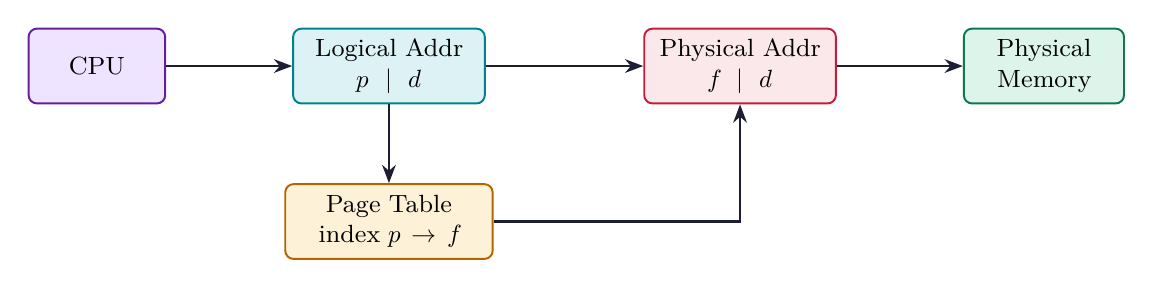
\begin{tikzpicture}[node distance=1.1cm and 2.0cm, thick, font=\small]
  \node[block, text width=1.5cm, fill=hdrpurple, draw=mypurple] (cpu) {CPU};
  \node[block, right=1.6cm of cpu, text width=2.2cm, fill=hdrteal, draw=myteal] (logical) {Logical Addr\\$p \ \ | \ \ d$};
  \node[block, below=1.0cm of logical, text width=2.4cm, fill=hdramber, draw=myamber] (ptable) {Page Table\\index $p \to f$};
  \node[block, right=2.0cm of logical, text width=2.2cm, fill=hdrred, draw=myred] (physical) {Physical Addr\\$f \ \ | \ \ d$};
  \node[block, right=1.6cm of physical, text width=1.8cm, fill=hdrgreen, draw=mygreen] (ram) {Physical\\Memory};

  \draw[arrow] (cpu) -- (logical);
  \draw[arrow] (logical.south) -- ++(0, -0.2) -| (ptable.north);
  \draw[arrow] (ptable.east) -| (physical.south);
  \draw[arrow] (logical.east) -- (physical.west);
  \draw[arrow] (physical) -- (ram);
\end{tikzpicture}
\end{tcolorbox}

\begin{itemize}[leftmargin=*, itemsep=3pt]
  \item \textbf{TLB (Translation Lookaside Buffer):} A fast hardware cache of associative registers used to store recent page-to-frame translations. It reduces the memory access penalty from two cycles (one for page table, one for data) to close to one cycle.
\end{itemize}

\subsection{Segmentation}
Segmentation is a memory-management scheme that supports the programmer's view of memory. A logical address space is a collection of variable-length segments (e.g., main program, procedure, stack, variables).
\begin{itemize}[leftmargin=*, itemsep=3pt]
  \item \textbf{Segment Table:} Maps logical address $\langle \text{segment\_number}, \text{offset} \rangle$ to physical addresses. Each entry has a \textbf{base} (start physical address) and \textbf{limit} (length of segment).
\end{itemize}

% ===============================================================================
\section{Virtual Memory and Demand Paging}
% ===============================================================================

\textbf{Virtual Memory} allows execution of processes that are not completely in main memory. It enables extremely large logical address spaces.

\subsection{Demand Paging \& Page Faults}
Pages are loaded into RAM only when they are referenced during execution (lazy swapper).
\begin{itemize}[leftmargin=*, itemsep=3pt]
  \item \textbf{Page Table Entry:} Includes a \textbf{valid-invalid bit} ($V/I$). $V$ means page is in memory; $I$ means page is on disk.
  \item \textbf{Page Fault:} Occurs when a running process references a page marked as invalid.
  \item \textbf{Page Fault Handling Sequence:}
\end{itemize}
  1. Trap to OS on page fault.
  2. Save process registers and state.
  3. Verify reference is valid, find page location on disk.
  4. Read page from disk into a free frame (using a page replacement algorithm if no free frames exist).
  5. Update page table (set bit to $V$).
  6. Restart the instruction that was interrupted by the trap.

\subsection{Page Replacement Algorithms}
When no frames are free, the OS must swap a page out to make room.
\begin{itemize}[leftmargin=*, itemsep=3pt]
  \item \textbf{FIFO (First-In, First-Out):} Replaces the oldest page. Prone to \textbf{Belady's Anomaly} --- page fault rate increases as physical frame allocation increases.
  \item \textbf{Optimal (OPT):} Replaces the page that will not be used for the longest time in the future. Optimal benchmark, but impossible to implement (requires future knowledge).
  \item \textbf{LRU (Least Recently Used):} Replaces the page that has not been referenced for the longest time in the past. Requires hardware support (counter or stack).
\end{itemize}

\subsection{Thrashing}
\textbf{Thrashing} is a state where a process spends more time paging (swapping pages in and out of disk) than executing useful instructions.
\begin{itemize}[leftmargin=*, itemsep=3pt]
  \item \textbf{Cause:} The process has been allocated fewer frames than its \textbf{working set} (the set of pages it is actively using). As a result, it page faults immediately, forcing page swaps in a continuous loop.
  \item \textbf{Solution:} Working-Set Model (allocates frames based on active page locality) or Page-Fault Frequency (PFF) control.
\end{itemize}

\newpage
% ===============================================================================
% MANDATORY QUICK REVISION PAGE
% ===============================================================================
\begin{center}
  {\large\bfseries\color{myred} Quick Revision --- Module 6}\\[3pt]
  {\small\color{mydark} Memory Management $|$ OE-EC604B}
\end{center}
\noindent{\color{myred}\rule{\linewidth}{1.2pt}}
\vspace{4pt}

\begin{tcolorbox}[formulabox, title={\textbf{Virtual Memory Math}}]
$$\text{Effective Access Time (EAT)} = (1 - p) \times T_{\text{mem}} + p \times T_{\text{fault}}$$
where $p$ = Page Fault Rate ($0 \le p \le 1$), $T_{\text{mem}}$ = RAM Access Time, $T_{\text{fault}}$ = Page Fault Service Time (disk seek + read).
\end{tcolorbox}

\begin{tcolorbox}[defbox, title={\textbf{One-Line Definitions}}]
\begin{itemize}[leftmargin=*, itemsep=2.5pt, topsep=0pt]
  \item \textbf{Internal Fragmentation:} Wasted memory inside a fixed partition allocated to a smaller process.
  \item \textbf{External Fragmentation:} Free memory blocks distributed non-contiguously, preventing allocation.
  \item \textbf{Paging:} Non-contiguous allocation breaking physical memory into fixed frames and logical into pages.
  \item \textbf{TLB:} Translation Lookaside Buffer; hardware cache to speed up logical-to-physical address mapping.
  \item \textbf{Segmentation:} Memory allocation method based on logical units (code, stack, global data).
  \item \textbf{Demand Paging:} Lazy page allocation technique loading pages only on execution references.
  \item \textbf{Belady's Anomaly:} Phenomenon where allocating more physical frames increases page faults in FIFO.
  \item \textbf{Thrashing:} System state where CPUs sit idle because processes are locked in page-swap loops.
\end{itemize}
\end{tcolorbox}

\begin{tcolorbox}[exambox, title={\textbf{Frequently Asked / Viva Questions}}]
\begin{enumerate}[topsep=0pt, label=\textbf{Q\arabic*.}, itemsep=5pt]
  \item \Q{Compare Paging and Segmentation.}
    Paging divides memory into fixed-size blocks (pages/frames), avoiding external fragmentation but suffering from internal fragmentation. It is invisible to the user. Segmentation divides memory into logical variable-size modules, matching the programmer's view, but suffers from external fragmentation.
  \item \Q{Given a reference string: \texttt{7, 0, 1, 2, 0, 3, 0, 4, 2, 3}. Frame size = 3.}\\
    \textbf{Calculate page faults for: (a) FIFO, (b) LRU, (c) Optimal.}\par
    *(a) FIFO:* Frames status:\par
    - Ref 7: [7] - Fault 1\par
    - Ref 0: [7, 0] - Fault 2\par
    - Ref 1: [7, 0, 1] - Fault 3\par
    - Ref 2: [2, 0, 1] (replaces 7) - Fault 4\par
    - Ref 0: [2, 0, 1] - Hit\par
    - Ref 3: [2, 3, 1] (replaces 0) - Fault 5\par
    - Ref 0: [2, 3, 0] (replaces 1) - Fault 6\par
    - Ref 4: [4, 3, 0] (replaces 2) - Fault 7\par
    - Ref 2: [4, 2, 0] (replaces 3) - Fault 8\par
    - Ref 3: [4, 2, 3] (replaces 0) - Fault 9. \textbf{Total Faults = 9.}\par
    *(b) LRU:* Frames status:\par
    - Ref 7, 0, 1: [7, 0, 1] - Faults = 3\par
    - Ref 2: [2, 0, 1] (replaces 7) - Fault 4\par
    - Ref 0: [2, 0, 1] - Hit (0 is most recent)\par
    - Ref 3: [2, 0, 3] (replaces 1) - Fault 5\par
    - Ref 0: [2, 0, 3] - Hit\par
    - Ref 4: [4, 0, 3] (replaces 2) - Fault 6\par
    - Ref 2: [4, 0, 2] (replaces 3) - Fault 7\par
    - Ref 3: [3, 0, 2] (replaces 4) - Fault 8. \textbf{Total Faults = 8.}\par
    *(c) Optimal:* Frames status:\par
    - Ref 7, 0, 1: [7, 0, 1] - Faults = 3\par
    - Ref 2: [2, 0, 1] (replaces 7, unused furthest) - Fault 4\par
    - Ref 0: [2, 0, 1] - Hit\par
    - Ref 3: [2, 0, 3] (replaces 1, unused furthest) - Fault 5\par
    - Ref 0: [2, 0, 3] - Hit\par
    - Ref 4: [4, 0, 3] (replaces 2, unused furthest) - Fault 6\par
    - Ref 2: [2, 0, 3] (replaces 4) - Fault 7\par
    - Ref 3: [2, 0, 3] - Hit. \textbf{Total Faults = 7.}
  \item \Q{What is Belady's Anomaly? Give an example of when it occurs.}
    Belady's Anomaly is when allocating more page frames to a process increases the number of page faults. It occurs in FIFO page replacement. Example string: \texttt{1, 2, 3, 4, 1, 2, 5, 1, 2, 3, 4, 5}. Frame size = 3 gives 9 faults; Frame size = 4 gives 10 faults.
  \item \Q{What is a TLB and how does it improve Effective Access Time?}
    A TLB is a fast associative cache on the CPU containing translation table entries. Instead of doing two memory accesses (one for page table in RAM, one for target location), the CPU checks the TLB. If it's a hit, the translation is resolved in $< 1$ cycle, minimizing EAT.
  \item \Q{Explain the concept of compaction in memory management.}
    Compaction is a technique used to resolve external fragmentation in variable partitioning. The OS dynamically shifts active processes in memory to make them contiguous, merging all small free holes into a single large free partition.
  \item \Q{What is thrashing? How can it be detected and prevented?}
    Thrashing occurs when a process is constantly swapping pages in and out of disk because it has been allocated fewer frames than its active working set. Detected when CPU utilization drops and disk queuing spikes. Prevented using the Working-Set Model or Page-Fault Frequency controls.
  \item \Q{Describe the page fault handling mechanism.}
    Process references page $\to$ MMU detects invalid bit $\to$ traps to OS kernel $\to$ OS checks virtual address and finds page on disk $\to$ allocates free frame $\to$ schedules I/O to read page $\to$ updates page table to valid $\to$ resumes the process.
  \item \Q{How does logical address space differ from physical address space?}
    Logical address space is the set of all virtual addresses generated by a program during compilation/execution. Physical address space is the set of actual physical hardware addresses in main memory (RAM).
  \item \Q{Explain the difference between internal and external fragmentation.}
    Internal fragmentation occurs when allocated memory is slightly larger than the process's demand, leaving wasted space inside the partition. External fragmentation occurs when free memory is sufficient but broken into small, non-contiguous blocks.
  \item \Q{What is a dirty bit (modify bit) and how does it optimize page replacement?}
    A dirty bit is a flag set in the page table entry when a page is written to. During page replacement, if the dirty bit is 0 (page unchanged), the OS can overwrite the frame without writing it back to disk, halving page-fault overhead.
\end{enumerate}
\end{tcolorbox}

\begin{tcolorbox}[tikzbox, title={Page Replacement Algorithms summary}]
\renewcommand{\arraystretch}{1.4}
\par\noindent
\begin{tabularx}{\linewidth}{|B{2.2cm}|>{\small\centering\arraybackslash}X|>{\small\centering\arraybackslash}X|>{\small\centering\arraybackslash}X|}
\hline
\textbf{Algorithm} & \textbf{\color{myred}Implementation Complexity} & \textbf{\color{myteal}Hardware Support?} & \textbf{\color{myamber}Belady's Anomaly?} \\
\hline
\textbf{FIFO} & Very Low & None & Yes \\
\hline
\textbf{Optimal} & Impossible (needs future data) & None & No \\
\hline
\textbf{LRU} & High (requires stacks/counters) & Yes (clock/reference bits) & No \\
\hline
\end{tabularx}
\end{tcolorbox}

\end{document}
